\chapter{Introducci\'on}

%tesis en linguistica http://elies.rediris.es/miscelanea/misce_9/alcina.pdf

En este cap\'itulo daremos una introducci\'on al problema de la generaci\'on autom\'atica de expresiones referenciales, contaremos las contribuciones de este trabajo y mostraremos como esta organizada la tesis.\\

La generaci\'on de lenguaje natural (GLN) es el proceso de la construcci\'on de un texto en lenguaje natural para la comunicaci\'on con fines espec\'ificos. Esta es una rama principal de la inteligencia artificial.\\

La generaci\'on autom\'atica de expresiones referenciales es una sub\'area de la generaci\'on de lenguaje natural.\\

Cuando hablamos, nos referimos a cosas, estas referencias, son expresiones referenciales, un sistema que genera texto, tambi\'en deber\'a generar expresiones referenciales.\\


Un sistema de generaci\'on autom\'atica de texto en lenguaje natural deber\'ia incluir m\'inimamante 
las tareas de determinaci\'on del contenido (que decir), lexicalizaci\'on (con que palabras), y la realizaci\'on ling\"{u}\'istica (armar el  sintagma nominal para que sea gramaticalmente correcto). \\


Esto mismo se aplica a la generaci\'on autom\'atica de expresiones referenciales, en la cual tendremos que la determinaci\'on de contenido estar\'a dada por las propiedades del objeto que queremos nombrar, la lexicalicalizaci\'on, las palabras que queremos usar para nombrarlo, y la realizaci\'on ling\"u\'istica, armar el sintagma nominal para que sea gramaticalmente correcto.\\

 


%Incluso la tarea de agregaci\'on puede argumentar que forme parte de la generaci\'on de una descripci\'on distintiva, como el contenido sem\'antico de alguna fuerza
%casos m\'as se reparten entre varios sintagmas nominales parcialmente distintivas

 %The domain defines the types of entities that are being referred to, in some
%cases even a particular set of entities with all their properties. A
%context set
%contains a subset of the domain entities, for example, the landmarks visible at a certain point of the path for which we are giving directions, a
%subset of the photographs used in an experimental setup, or the cooking ingredients that have already been mentioned in a recipe. In a visual environment, the context set, including the
%properties of its member objects and their spatial configuration, is often called  a scene.Document Planning, Microplanning and Realisation  A system charged
%with generating a fully- edged natural language description will as a minimum
%have to perform the tasks of content determination (selecting the properties of the
%target referent to be mentioned), lexicalisation (choosing the words to represent
%the properties), and linguistic realisation (constructing a grammatically correct
%noun phrase). Even the task of aggregation can be argued to form part of the
%generation of a distinguishing description, as the semantic content might in some
%cases best be spread across several partially distinguishing noun phrases

\begin{figure}[ht]
\centering
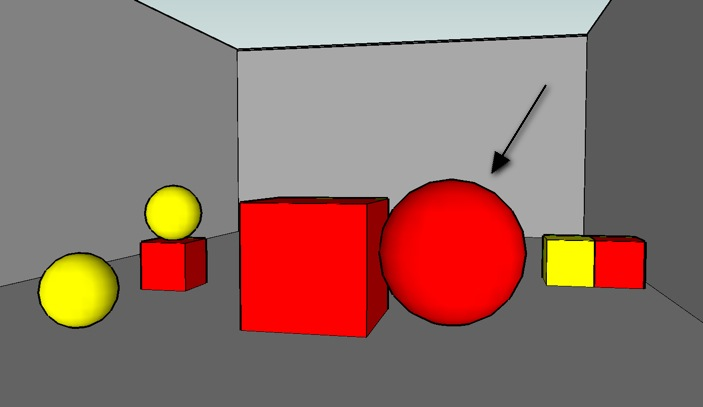
\includegraphics[width=0.6\textwidth]{images/22sinletras.jpg}
\caption{Ejemplo de contexto}
\label{GRE3D7-stimulus1}
\end{figure}


Supongamos que uno quiere se\~nalar un objeto de la Figura~\ref{GRE3D7-stimulus1} a un destinatario. La mayor\'{i}a de las personas
no tendr\'a dificultad en realizar esta tarea, mediante la producci\'on de una expresi\'on referencial como ``la
esfera roja al lado del cubo rojo'', por ejemplo. \\

\begin{figure}[ht]
\centering
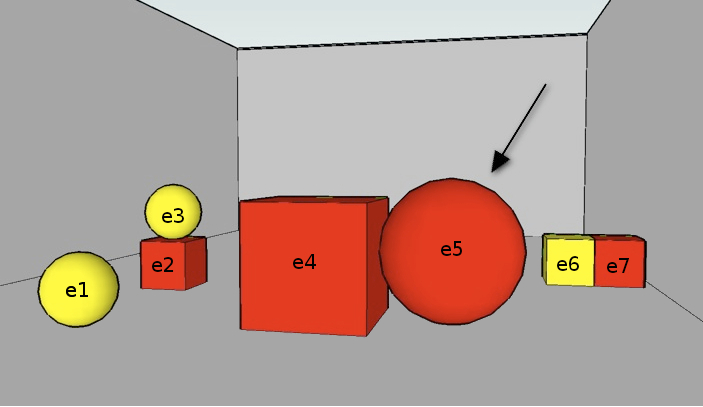
\includegraphics[width=0.6\textwidth]{images/22.jpg}
\caption{Ejemplo de contexto con objetos etiquetados}
\label{GRE3D7-stimulus2}
\end{figure}

Ahora imagine una computadora que se enfrenta a la misma
tarea, en principio la misma imagen no servir\'a a la computadora, ella necesita tener identificados los objetos y sus propiedades, como en Figura~\ref{GRE3D7-stimulus2}. Suponiendo que tiene acceso a una base de datos que contiene todas
las propiedades relevantes de los objetos de la escena, como se muestra en la figura, tiene que encontrar alguna
combinaci\'on de propiedades que se aplica \'unicamente a $e_5$, y no a los otros objetos.\\

Esta tarea de encontrar las propiedades que aplican a un objeto y no a los otros, se llama selecci\'on de contenido de una expresi\'on referencial.  \\

Imagine una computadora con un conjunto de propiedades de los objetos queriendo distinguir a $e_5$, puede que haya m\'as de una forma en la que $e_5$ puede ser distinguido del resto (``la esfera verde de la izquierda'', ``la peque\~na esfera verde'', ``la esfera sobre el cubo azul''), la computadora tiene que decidir cu\'al de esas expresiones referenciales es \'optima en el contexto dado. Por otra parte, el concepto de \'optimo puede significar diferentes cosas.\\

Se podr\'{i}a pensar, por ejemplo, que las referencias son \'optimas cuando son m\'{i}nimas en longitud,
que contiene s\'olo la informaci\'on suficiente para identificar el objeto target. Pero, como veremos, la b\'usqueda de referencias m\'{i}nimas
es computacionalmente cara, y no es necesariamente lo que los hablantes hacen, ni lo que es m\'as \'util para los oyentes.\\


%Suppose one wants to point out an object in Figure~\ref{GRE3D7-stimulus-graph} to an addressee. Most speakers
%have no difficulty in accomplishing this task, by producing a referring expression
%such as ``the green ball on the cube'' for example. Now imagine a computer being confronted
%with the same task, aiming to point out individual $e3$. Assuming it has access to a
%database containing all the relevant properties of the objects in the scene as shown in the figure, it needs to
%find some combination of properties which applies to $e3$, and not to the other objects.
%There is a choice though: There are many ways in which $e3$ can be set apart from the
%rest (``the green ball on the left'', ``the small green ball'', ``the ball on the blue cube''), and
%the computer has to decide which of these is optimal in the given context. Moreover,
%optimality can mean different things. It might be thought, for instance, that references
%are optimal when they are minimal in length, containing just enough information to
%single out the target. But, as we shall see, finding minimal references is computationally
%expensive, and it is not necessarily what speakers do, nor what is most useful to hearers.

Entonces,  ?`qu\'e es la Generaci\'on de Expresiones referenciales? \\
%Las expresiones referenciales juegan un papel central
%en la comunicaci\'on, y se han estudiado ampliamente en muchas ramas (computacionales) de la ling\"u\'{i}stica,
 %incluyendo Generaci\'on del Lenguaje Natural (NLG). NLG 

Es el proceso de convertir autom\'aticamente la informaci\'on no ling\"u\'{i}stica (por ejemplo, a partir de una base de datos como se ha ilustrado en nuestra figura) a texto en lenguaje natural, que es \'util para aplicaciones pr\'acticas que van desde la generaci\'on de pron\'osticos del tiempo, a resumir informaci\'on m\'edica~\cite{dale2000}. \\

De todas las subtareas de NLG, la Generaci\'on de Expresiones Referenciales (GER) es
una de las que han recibido m\'as atenci\'on. En la pr\'actica, la mayor\'ia de los
sistemas NLG, con independencia de su finalidad,
contiene un m\'odulo GER de alg\'un tipo~\cite{Mellish2004}. Esto no es sorprendente
en vista del papel central que las expresiones referenciales en la comunicaci\'on. Un sistema que proporciona
consejos sobre los viajes a\'ereos (White, Clark y Moore 2010) ha de hacer referencia a los vuelos (``el
vuelo m\'as barato'', ``un vuelo directo''), un sistema de navegaci\'on para autom\'oviles~\cite{Drager:2012:GLN:2380816.2380908}
necesita para generar descripciones espaciales para las \'areas (``tomar el puente junto a la iglesia a la derecha''),
y un sistema de di\'alogo de un robot que ensambla piezas de juguetes, junto con un usuario humano~\cite{foster-etal-ijcai2009} ha de hacer referencia a los componentes (``inserte el perno verde hasta el final en el cubo rojo'').\\
%So, what is Referring Expression Generation? Referring expressions play a central role
%in communication, and have been studied extensively in many branches of (computational) linguistics,
% including Natural Language Generation (NLG). NLG is concerned with the process of automatically converting non-linguistic information (e.g.,
%from a database such as the one illustrated in our figure) into natural language text, which is useful for practical applications
%ranging from generating weather forecasts to summarizing medical information~\cite{dale2000}. Of all the subtasks of NLG, Referring Expression Generation (REG) is
%among those that have received most scholarly attention. A survey of implemented,
%practical NLG systems shows that virtually all of them, regardless of their purpose,
%contain an REG module of some sort~\cite{Mellish2004}. This is hardly surprising
%in view of the central role that reference plays in communication. A system providing
%advice about air travel (White, Clark, and Moore 2010) needs to refer to flights (``the
%cheapest flight'' ``the KLM direct flight''), an in-car navigation system~\cite{Drager:2012:GLN:2380816.2380908}
%needs to generate spatial descriptions for areas (``take the bridge next to the church on your right''), 
%and a robot dialogue system that assembles construction
%toys together with a human user~\cite{foster-etal-ijcai2009} needs to refer to the components
%(``insert the green bolt through the end of this red cube'').




El dominio define los tipos de entidades que est\'an siendo contemplados, en algunos
casos incluso un determinado conjunto de entidades con todas sus propiedades.\\

El contexto contiene un subconjunto de las entidades del dominio, por ejemplo, los puntos de referencia visibles en un cierto punto de la ruta para la que estamos dando direcciones, un
subconjunto de las fotograf\'ias utilizadas en una configuraci\'on experimental, o los ingredientes de cocina que ya se han mencionado en una receta. En un entorno visual, el contexto, incluyendo las
propiedades de sus objetos y su configuraci\'on espacial, se puede llamar escena. \\

El \emph{target} u objetivo, es el objeto al cual queremos referirnos. En las escenas de nuestros ejemplos es el se\~nalado por la flecha.\\

Los \emph{distractores} son objetos los cuales se encuentran en el contexto considerado, y por los cuales es necesario hacer una expresi\'on referencial para identificar a nuestro target. \\

En esta tesis estudiamos la generaci\'on autom\'atica de expresiones referenciales, 
primero mostramos c\'omo podemos a\~nadir no determinismo (posibilidad de dar distantas expresiones referenciales considerando el mismo contexto y target) de los algoritmos de refinamiento estudiados, ellos tienen un orden fijo en el cual consideran las propiedades y relaciones, y la naturalidad de las expresiones referenciales que generan dependen de este orden particular considerado, nosotros proponemos reemplazar ese orden fijo
sobre las propiedades y/o relaciones de la escena de entrada por una~\emph{probabilidad de uso} para cada propiedad y/o relaci\'on, y modificar el algoritmo para que tenga en cuenta esas propiedades.\\

De esta manera, cada llamada al algoritmo puede producir diferentes ERs para la misma escena y target de entrada. \\

Nuestra aproximaci\'on es emp\'irica, en el sentido de que para evaluar nuestros resultados, usaremos corpus (colecciones de datos) de expresiones referenciales hechas por humanos. \\

Es decir nuestra meta, no s\'olo ser\'a crear algoritmos para la generaci\'on autom\'atica de expresiones referenciales, sino crearlos de tal manera que podamos imitar en gran medida lo que dir\'ian las personas.\\

Mostraremos que dado un corpus adecuado (como el corpus GRE3D7 el cual introduciremos en Cap\'itulo \ref{sec:seleccion}) o el corpus TUNA del cual hablaremos en Cap\'itulo~\ref{sec:seleccion} podemos estimar estas probabilidades de uso de manera que las ER se generen con una distribuci\'on de probabilidad que coincide en gran medida con las que se encuentra en el corpus.\\

%Todos los algoritmos GER requieren una lista de propiedades que se pueden utilizar para describir los objetos en la escena, esta lista tiene un orden, y la naturalidad de las ERs generadas depende fuertemente de este ordenamiento.\\

%Our goal is actually twofold. First we show how we can add non-determinism to the refinement algorithms, by replacing the fixed ordering 
%over the properties of the input scene by a \emph{probability of use} for each property, and modifying the algorithm accordingly.  
%In this way, each call to the algorithm can produce different REs for the same input scene and target.  We will then show that given suitable corpora of REs (like the GRE3D7 corpora discussed in~\cite{viet:gene11}) or the TUNA corpus introduced in~\cite{gatt-balz-kow:2008:ENLG} we can estimate these probability of use so that REs are generated with a probability distribution that matches those found in the corpora.  

%All REG algorithms require an 
%ordered list of properties that can be used to described the objects in the scene, and the naturalness of the generated REs strongly depends on this ordering. 
%coverage results reported over Viethen and 
%Dale's cabinet corpus means that \emph{some ordering} produces a reasonably wide coverage.  In other words, it has been shown that refinement algorithms have the capacity of producing REs similar to those produced by human subjects, provided a suitable ordering over relations appearing 
%in the input scene is available, but it is unclear which of all possible orders should be used.  In this article we directly address this issue.  
%The goal of this paper is twofold. First we show how we can add non-determinism and overspecification to the refinement algorithms, by replacing the fixed ordering 
%over properties of the input scene by a \emph{probability of use} for each property, and modifying the algorithm accordingly.  
%In this way, each call to the algorithm can produce different REs for the same input scene and target.  We will then show that given suitable corpora of REs (like the GRE3D7 corpora discussed in~\cite{viet:gene11}) we can estimate these probabilities of use so that REs are generated with a probability distribution that matches the one found in corpora.  

\cite{arec2:2008:Areces}~mostraron que el algoritmo de refinamiento utilizando el lenguaje de descripci\'on \el como lenguaje formal es capaz de generar 67\% de
las ERs relacionales en el corpus ~\cite{viethen06:_algor_for_gener_refer_expres} cuando se consideran todos los posibles \'ordenes de las relaciones en el dominio. Esto est\'a en marcado contraste con el an\'alisis hecho en~\cite{viethen06:_algor_for_gener_refer_expres} sobre el cabinet corpus, de algoritmos basados en la propuesta original Dale y de Reiter.\\

%show that the refinement algorithm using the description language \el as formal language is capable of generating 67\% of 
%the relational REs in the~\cite{viethen06:_algor_for_gener_refer_expres} dataset, when all possible orders of the relations in the domain are considered. This is in sharp contrast with the analysis 
%done in~\cite{viethen06:_algor_for_gener_refer_expres} over the cabinet corpus, of algorithms based in Dale and Reiter's original proposal.    

%As mentioned, refinement algorithms require an 
%ordered list of the properties that can be used to described the objects in the scene, and the coverage results reported over Viethen and 
%Dale's cabinet corpus means that \emph{some ordering} produces a reasonably wide coverage.  In other words, it has been shown that refinement algorithms have the capacity of producing REs similar to those produced by human subjects, provided a suitable ordering over relations appearing 
%in the input scene is available, but it is unclear which of all possible orders should be used.  In this article we directly address this issue.  

Los resultados de cobertura reportados sobre Viethen and 
Dale's sobre el Cabinet corpus significan que~\emph{alg\'un orden} produce una razonablemente amplia cobertura. En otras palabras, se ha demostrado que los algoritmos de refinamiento tienen la capacidad de producir ERs similares a los producidos por los humanos, proporcionado una ordenaci\'on adecuada sobre las relaciones que aparecen
en la escena de entrada, pero no est\'a claro cu\'al de todos los \'ordenes posibles se debe utilizar. En esta tesis abordamos directamente esta cuesti\'on.

% In Section~\ref{sec:algorithm} we introduce the technical details of the 
%refinement algorithms presented in~\cite{arec2:2008:Areces,arec:usin11} and show how to introduce non-determinism using 
%the probability of use of the properties in the input scene. In this section, we assume that these probabilities are provided as 
%input to the algorithm. In Section~\ref{sec:learning}, we show how to estimate the 
%probability of use of a property from training data. Given corpora consisting of pairs (scene, target) together with the REs used to 
%describe the target in each case, we propose a method to compute the probability of use of each property for each scene, and use a machine learning approach to generalize these properties to new targets and scenes not appearing in the corpora. 

%Testing of the resulting algorithms shows that there is still one factor missing to property account for the REs found in corpora: overspecification.  Refinement algorithms only allow a mild form of over-specification in the REs produced.  We discuss this in 
%Section~\ref{sec:overspecification} and propose a modification that let the algorithm generate overspecified, but non trivially redundant RE.  The modification proposed is inspired by the work of~\cite{keysar:Curr98}, on the egocentric basis of language.  
%Section~\ref{sec:evaluation} presents a quantitative evaluation of the resulting algorithm and discusses interesting examples \textit{over the GRE3D7 and the TUNA-corpus}. 
%We show that when trained with scenes from the GRE3D7 corpora the algorithm can generate REs with a probability distribution that, 
%in certain scenes, coincides with an up to 84.49\% of accuracy with the probability distribution of REs used by humans for that scene. 
%\textit{We compare our results with the TUNA-corpus with results of the ASGRE challenge and show better results than the adquire for the best system in 2008.
%In Section~\ref{sec:error} we show an interesting analysis of errors that can be taken into account in the next works.}, then in Section~\ref{sec:related-work} we describe related work in the area.

%In Section~\ref{sec:discussion} we discuss motivations and future lines of research, focusing on recent work discussing the role 
%of non-determinism and over-specification in the generation of referring expressions. 

\section{Descripci\'on del problema}
\label{sec:intro}

En ling\"u\'{i}stica, una expresi\'on referencial ER (que viene de la expresi\'on en ingl\'es referring expression (RE)) es una expresi\'on que identifica un\'ivocamente a un objeto para un interlocutor particular, desde un conjunto de posibles distractores. Por ejemplo si nosotros queremos identificar a un cierto animal d de un conjunto de mascotas, la expresi\'on ``el perro'' ser\'a ER si d es el \'unico perro en el conjunto, y si nosotros estamos seguros que nuestro interlocutor identificar\'a a d como un perro. Para una persona esto ser\'ia una tarea f\'acil de realizar, pensemos ahora como lo har\'ia una computadora, supongamos que queremos conseguir un algoritmo que genere autom\'aticamente esas expresiones referenciales que la gente genera.\\

Una propiedad es una caracter\'istica de una entidad particular por ejemplo, la raza de un perro, el tener o no tener bigotes para un hombre, o el color para un objeto, cada entidad puede tener muchas propiedades, e incluso puede tener relaciones, as\'i como las relaciones familiares, las relaciones con respecto a la posici\'on f\'isica, por ejemplo: el hecho de estar situado al lado de otro obejto.\\

 Para que una computadora pueda generar las ER generadas por las personas, primero deber\'ia seleccionar las propiedades y/o relaciones que se incluir\'an en la RE, deber\'a tener una base de datos conteniendo las propiedades y relaciones relevantes de la escena, podemos imaginar que una computadora podr\'a generar muchas m\'as expresiones referenciales que una persona, este es un desaf\'io que direccionaremos en esta tesis, nuestra meta ser\'a imitar al humano en la generaci\'on de expresiones referenciales. \\

Esta selecci\'on de la ER m\'as apropiada tambi\'en debe tener en cuenta al interlocutor, es natural que los humanos demos distintas ER a distintos interlocutores. En el \'area muchas veces se habla de optimalidad de la RE, pero con diferentes significados, para algunos una ER \'optima es aquella que dice lo m\'inimo necesario para identificar al objeto target, para otros es la menos esfuerzo requiere del interlocutor para identificarlo.\\
%Usamos generaci\'on de ER todo el tiempo en la vida real, y as\'i los sistemas tambi\'en las usan, por lo tanto son necesarios los algoritmos para generarlas autom\'aticamente, las ER han sido estudiadas y tienen muchas aplicaciones pr\'acticas desde generaci\'on de reportes meteorol\'ogicos a generaci\'on autom\'atica de res\'umenes de informaci\'on m\'edica~\cite{dale2000}. Muchos sistemas de GLN incluyen un m\'odulo de GER~\cite{Mellish2004}.
%Las expresiones referenciales ocupan un papel central en la comunicaci\'on, popr ejemplo sistemas que proveen advertencias en navegaci\'on aerea
 %(White, Clark, and Moore 2010) necesitan referirse a los vuelos, en sistemas de navegaci\'on en auto~\cite{Drager:2012:GLN:2380816.2380908} se necesitan generar descripciones espaciales para \'areas (tomar la siguiente calle a la derecha de la iglesia), y sistemas de di\'alogo con un robot que ensambla piezas para la contrucci\'on de juguetes~\cite{foster-etal-ijcai2009} necesita referirse a las piezas (insert\'a el tornillo verde en el cubo)

%Our goal is actually twofold. First we show how we can add non-determinism to the
%refinement algorithms, by replacing the fixed ordering over the properties of the input scene
%by a probability of use for each property, and modifying the algorithm accordingly. In this
%way, each call to the algorithm can produce different REs for the same input scene and
%target. We will then show that given suitable corpora of REs (like the GRE3D7 corpora
%discussed in (Viethen, 2011)) ot the TUNA corpus introduced in (Gatt et al., 2008) we can
%estimate these probability of use so that REs are generated with a probability distribution
%that matches those found in the corpora.
%All REG algorithms require an ordered list of properties that can be used to described
%the objects in the scene, and the naturalness of the generated REs strongly depends on this
%ordering.
%(Areces et al., 2008) show that the refinement algorithm using the description language
%EL as formal language is capable of generating 67\% of the relational REs in the (Viethen &
%Dale, 2006) dataset, when all possible orders of the relations in the domain are considered.
%This is in sharp contrast with the analysis done in (Viethen & Dale, 2006) over the cabinet
%corpus, of algorithms based in Dale and Reiter's original proposal.
%As mentioned, refinement algorithms require an ordered list of the properties that can
%be used to described the objects in the scene, and the coverage results reported over Viethen
%and Dale's cabinet corpus means that some ordering produces a reasonably wide coverage.
%In other words, it has been shown that refinement algorithms have the capacity of producing
%REs similar to those produced by human subjects, provided a suitable ordering over relations
%appearing in the input scene is available, but it is unclear which of all possible orders should
%be used. In this article we directly address this issue.
%The rest of the paper is structured as follows. In Section 3 we introduce the technical
%details of the refinement algorithms presented in (Areces et al., 2008, 2011) and show how
%to introduce non-determinism using the probability of use of the properties in the input
%scene. In this section, we assume that these probabilities are provided as input to the
%algorithm. In Section 4, we show how to estimate the probability of use of a property from
%training data. Given corpora consisting of pairs (scene, target) together with the REs used
%to describe the target in each case, we propose a method to compute the probability of use
%of each property for each scene, and use a machine learning approach to generalize these
%properties to new targets and scenes not appearing in the corpora.
%Testing of the resulting algorithms shows that there is still one factor missing to prop-
%erty account for the REs found in corpora: overspecification. Refinement algorithms only
%allow a mild form of over-specification in the REs produced. We discuss this in Section 5
%and propose a modification that let the algorithm generate overspecified, but non trivially
%redundant RE. The modification proposed is inspired by the work of (Keysar et al., 1998),
%on the egocentric basis of language. Section 6 presents a quantitative evaluation of the
%resulting algorithm and discusses interesting examples over the GRE3D7 and the TUNA-
%corpus. We show that when trained with scenes from the GRE3D7 corpora the algorithm
%can generate REs with a probability distribution that, in certain scenes, coincides with an
%up to 84.49\% of accuracy with the probability distribution of REs used by humans for that
%scene. We compare our results with the TUNA-corpus with results of the ASGRE challenge
%and show better results than the adquire for the best system in 2008. In Section 7 we show
%an interesting analysis of errors that can be taken into account in the next works., then in
%Section 8 we describe related work in the area.
%In Section 9 we discuss motivations and future lines of research, focusing on recent work
%discussing the role of non-determinism and over-specification in the generation of referring
%expressions.

%Suppose one wants to point out an object in Figure~\ref{GRE3D7-stimulus-graph} to an addressee. Most speakers
%have no difficulty in accomplishing this task, by producing a referring expression
%such as ``the green ball on the cube'' for example. Now imagine a computer being confronted
%with the same task, aiming to point out individual $e3$. Assuming it has access to a
%database containing all the relevant properties of the objects in the scene as shown in the figure, it needs to
%find some combination of properties which applies to $e3$, and not to the other objects.
%There is a choice though: There are many ways in which $e3$ can be set apart from the
%rest (``the green ball on the left'', ``the small green ball'', ``the ball on the blue cube''), and
%the computer has to decide which of these is optimal in the given context. Moreover,
%optimality can mean different things. It might be thought, for instance, that references
%are optimal when they are minimal in length, containing just enough information to
%single out the target. But, as we shall see, finding minimal references is computationally
%expensive, and it is not necessarily what speakers do, nor what is most useful to hearers.

%So, what is Referring Expression Generation? Referring expressions play a central role
%in communication, and have been studied extensively in many branches of (computational) linguistics, including Natural Language Generation (NLG). NLG is concerned with the process of automatically converting non-linguistic information (e.g.,
%from a database such as the one illustrated in our figure) into natural language text, which is useful for practical applications
%ranging from generating weather forecasts to summarizing medical information~\cite{dale2000}. Of all the subtasks of NLG, Referring Expression Generation (REG) is
%among those that have received most scholarly attention. A survey of implemented,
%practical NLG systems shows that virtually all of them, regardless of their purpose,
%contain an REG module of some sort~\cite{Mellish2004}. This is hardly surprising
%in view of the central role that reference plays in communication. A system providing
%advice about air travel (White, Clark, and Moore 2010) needs to refer to flights (

%que es \'util para aplicaciones pr\'acticas
%que van desde la generaci\'on de pron\'osticos del tiempo para resumir la informaci\'on m\'edica (Reiter
%y Dale 2000). De todas las subtareas de NLG, referencia Generaci\'on Expresi\'on (REG) es
%entre los que han recibido mayor atenci\'on acad\'emica. Una encuesta de la marcha,
%sistemas pr\'acticos NLG muestra que pr\'acticamente todos ellos, independientemente de su finalidad,
%contener un m\'odulo REG de alg\'un tipo (Mellish et al. 2006). Esto no es sorprendente en
%habida cuenta del papel central que juega la referencia en la comunicaci\'on. Un sistema que proporciona
%consejos sobre los viajes a\'ereos (White, Clark, y Moore 2010), hay que hacer referencia a los vuelos (`` la
%m\'as barata de vuelo '', `` el vuelo directo KLM ''); un sistema de previsi\'on de polen (Turner et al.
%2008) tiene que generar descripciones espaciales para las \'areas con niveles bajos o altos de polen
%(`` el cintur\'on central y m\'as al norte ''), y un sistema de di\'alogo robot que re\'une
%juguetes de construcci\'on junto con un usuario humano (Giuliani et al 2010.), necesita para referirse a la
%componentes (`` insertar el perno verde hasta el final de este cubo rojo '').
%REG `` tiene que ver con la forma en que producimos una descripci\'on de una entidad que permite
%el oyente identificar esa entidad en un contexto dado '' (Reiter y Dale 2000, p\'agina 55).
%Dado que esto a menudo se puede hacer de muchas maneras diferentes, un algoritmo REG tiene que hacer una
%n\'umero de opciones. Seg\'un Reiter y Dale (2000), la primera opci\'on se refiere a lo
%forma
%de referirse expresi\'on es para ser utilizado; debe ser referido el objetivo de, por ejemplo,
%usando su propio nombre, un pronombre (`` \'el '') o una descripci\'on (`` el hombre con el lazo '').
%Los nombres propios han aplicabilidad limitada porque muchos objetos de dominio no tienen
%un nombre que es de uso com\'un. Para la generaci\'on de pronombre, un simple pero conservadora
%regla es discutido por Reiter y Dale (2000), similar al propuesto por Dale (1,989,
%p\'aginas 150 a 151): utilizar un pronombre si el objetivo fue mencionado en la frase anterior,
%y si esta frase conten\'ia ninguna referencia a cualquier otra entidad del mismo g\'enero.
%Reiter y Dale (2000) se concentran principalmente en la generaci\'on de descripciones. 
Para generar una expresi\'on referencial, se debe seleccionar el
conjunto de propiedades que distingue al objetivo (selecci\'on de contenidos), y c\'omo pueden las propiedades seleccionadas
convertirse en lenguaje natural (realizaci\'on ling\"u\'istica). La selecci\'on de contenido es un
complejo acto de equilibrio: tenemos que decir lo suficiente para permitir la identificaci\'on del objeto target, pero no demasiado. Una selecci\'on de la informaci\'on necesaria. Reiter y Dale discuten diversas estrategias que tratan de gestionar este
acto de equilibrio, basado en Dale y Reiter (1995), en ... que resume
y la compara varios algoritmos influyentes para la generaci\'on de descripciones.
creo que es esta cita.. pero no estoy segura (esto lo saque del survey...)
Dale, Robert and Ehud Reiter. 1995.
Computational interpretations of the
Gricean maxims in the generation of
referring expressions.
Cognitive Science

%which is useful for practical applications
%ranging from generating weather forecasts to summarizing medical information (Reiter
%and Dale 2000). Of all the subtasks of NLG, Referring Expression Generation (REG) is
%among the ones that have received most scholarly attention. A survey of implemented,
%practical  NLG  systems  shows  that  virtually  all  of  them,  regardless  of  their  purpose,
%contain a REG module of some sort (Mellish et al. 2006). This is hardly surprising in
%view  of  the  central  role  that  reference  plays  in  communication.  A  system  providing
%advice about air travel (White, Clark, and Moore 2010), needs to refer to flights (``the
%cheapest  flight'',  ``the  KLM  direct  flight'');  a  Pollen  forecast  system  (Turner  et  al.
%2008)  needs  to  generate  spatial  descriptions  for  areas  with  low  or  high  pollen  levels
%(``the  central  belt  and  further  North''),  and  a  robot  dialogue  system  that  assembles
%construction toys together with a human user (Giuliani et al. 2010), needs to refer to the
%components (``insert the green bolt through the end of this red cube'').
%REG ``is concerned with how we produce a description of an entity that enables
%the hearer to identify that entity in a given context'' (Reiter and Dale 2000, page 55).
%Since this can often be done in many different ways, a REG algorithm needs to make a
%number of choices. According to Reiter and Dale (2000), the first choice concerns what
%form
%of referring expression is to be used; should the target be referred to, for instance,
%using  its  proper  name,  a  pronoun  (``he'')  or  a  description  (``the  man  with  the  tie'').
%Proper  names  have  limited  applicability  because  many  domain  objects  do  not  have
%a name that is in common usage. For pronoun generation, a simple but conservative
%rule  is  discussed  by  Reiter  and  Dale  (2000),  similar  to  one  proposed  by  Dale  (1989,
%pages 150-151): use a pronoun if the target was mentioned in the previous sentence,
%and  if  this  sentence  contained  no  reference  to  any  other  entity  of  the  same  gender.
%Reiter  and  Dale  (2000)  concentrate  mostly  on  the  generation  of  descriptions.  If  the
%NLG  system  decides  to  generate  a  description,  two  choices  need  to  be  made:  which
%set of properties distinguishes the target (content selection), and how can the selected
%properties be turned into natural language (linguistic realisation). Content selection is a
%complex balancing act: we need to say enough to enable identification of the intended
%referent, but not too much. A selection of information needs to be made, and this needs
%to be done quickly. Reiter and Dale discuss various strategies that try to manage this
%balancing act, based on Dale and Reiter (1995), an early survey article that summarises
%and compares various influential algorithms for the generation of descriptions.
%
%\textcolor{blue}{traje esto...}
La selecci\'on de qu\'e propiedades y/o relaciones con otros objetos incluir en una expresi\'on referencial depender\'a del prop\'osito que tengamos para dicha expresi\'on referencial. Una expresi\'on referencial ser\'a muy distinta si nuestro objetivo es dar la m\'inima informaci\'on que identifique al objeto que si nuestro objetivo es ayudar al interlocutor a que identifique el objeto.\\

En la vida real hay muchas cosas que nos ayudan a darnos cuenta si nuestro interlocutor identific\'o el objeto target, como ser la expresi\'on de sorpresa nos dar\'ia una pauta de que no esta entendiendo lo que le queremos decir, pero cuando queremos hacer esa generaci\'on autom\'atica normalmente no poseemos esa clase de informaci\'on.\\

En esta tesis nos vamos a enfocar en la selecci\'on de contenidos de las expresiones referenciales, y el objetivo ser\'ia simular el comportamiento humano, para ello vamos a usar corpus de expresiones referenciales para aprender como realizan esta tarea las personas.\\

%concerned with the process of automatically converting non-linguistic information (e.g.,
%from a database) into natural language text, 
Un algoritmo para la generaci\'on autom\'atica de expresiones referenciales (GER), es un procedimiento que tomar\'a alg\'un tipo de input y dar\'a como resultado una expresi\'on referencial.\\


Cada objeto o entidad tiene un tipo, ciertas propiedades o caracter\'isticas y los valores de esas propiedades, que incluso pueden ser relaciones con otros objetos. \\

Por ejemplo: Que cosa es? (el tipo) Una esfera. Que color? Rojo. Esta al lado de otro objeto? Si. Cual? El cubo azul.\\

Con esta clase de datos para los objetos de la escena, tenemos una base de conocimento (KB), estos datos se pueden organizar en jerarqu\'ias, por ejemplo: conjunto de animales, conjunto de mamiferos, conjunto de insectos. Algunos conjuntos pueden estar contenidos en otros, es decir algunos objetos o entidades pueden compartir caracter\'isticas.\\

Si tenemos 100 caracter\'isticas de una persona, y con esas caracter\'isticas se pudiera identificar un\'ivocamente a una persona, un sistema que diera que las 100 caracter\'isticas no ser\'ia un sistema que suene muy natural, ya que una persona no dar\'ia 100 propiedades para identicar a una persona particular. As\'i podr\'iamos decir que las expresiones referenciales variaran seg\'un la cantidad de informaci\'on que dan, si dan la m\'inima informaci\'on para identificarlas un\'ivocamente ser\'an minimales, si dan m\'as informaci\'on estar\'an sobreespecificadas, pero en el caso de dar m\'as de la m\'inima informaci\'on... cu\'anta m\'as dar?\\

%El sistema deber\'ia tener una lista del orden de preferencia de los atributos a usar.\\ 

Para una persona identificar ciertos atributos puede ser m\'as f\'acil que identificar ciertos otros, por ejemplo cierto color verde podr\'{i}a ser m\'as complicado de identificar que el tama\~no. Notar que cuando decimos el tama\~no podemos decir ``grande'' y tenemos como marco de referencia a los objetos de la escena, en ese contexto un objeto es ``grande''.\\

Para un algoritmo entonces, ser\'ian cuestiones importantes de tener en cuenta:

\begin{itemize}
 \item Que propiedades o relaciones incluir?
 \item Cuando terminar (dar la expresi\'on minimal? o dar una expresi\'on sobreespecificada, si es sobreespecifica, que tan sobreespecificada?)
 \item Seguir un orden preferencias fijo para las propiedades? y luego otro para las relaciones?
 \item Hacer o no backtraking?
 \item Incluir o no negaciones?
\end{itemize}


Hay diferentes tipos de propiedades, por ejemplo taxon\'omicas (las que tiene el objeto, por ejemplo tipo, color), relacionales (las que necesitan dar una ER de otro objeto, por ejemplo ``estar al lado de...''), vagas (son las m\'as dificiles de identificar, ejemplo: chico, grande, no son propiedades absolutas), cuando usar un tipo u otro de propiedad... 
Si el objeto target tiene la propiedad de medir 1.80 de alto, y est\'a en un grupo donde los dem\'as son m\'as peque\~nos, es m\'as natural decir el m\'as alto, que el que mide 1.80.\\


%hablar de syntactic realization en algun lugar
%In many early REG proposals, Lexical Choice and Surface Realization follow Content
%Determination,  in  the  style  of  a  pipeline,  with  most  of  the  actual  research  focusing
%predominantly on Content Determination.

%Tambi\'en podemos hablar 
%
%to plurals, as in ``the old men and women'', where ``old'' may or may not pertain to the
%women. These issues have been studied in some detail as part of a systematic study of
%the ambiguities that arise in coordinated phrases of the form ``the Adjective Noun and
%Noun'',
Las primeras investigaciones en GER hicieron una serie de supuestos simplificadores, y como resultado los primeros
algoritmos GER s\'olo pod\'ian generar una variedad limitada de expresiones referenciales. Cuando
los investigadores comenzaron a levantar algunos de estos supuestos, esto di\'o lugar a algoritmos de GER
con un repertorio m\'as amplio, siendo capaces de generar, por ejemplo, plurales y expresiones relacionales. \\

Este movimiento ha creado una serie de nuevos desaf\'ios, sin embargo. Por ejemplo, el
n\'umero de formas en las que uno puede referirse a un conjunto de objetos de destino aumenta, por lo que la elecci\'on de una
buena expresi\'on referencial es m\'as dif\'icil.\\

Del mismo modo, incluso propuestas recientes tienden a asumir que no es problem\'atico para determinar qu\'e informaci\'on
es compartida entre el hablante y el oyente.
 (a) C\'omo se representa la informaci\'on del dominio?
(b) C\'omo se representa el contenido sem\'antico de una expresi\'on referencial ? y (c) C\'omo se pueden encontrar descripciones distintivas.\\

 En el contexto del corpus analizado en esta tesis, nos encontraremos con cuatro tipos diferentes de atributos:
tipos de objetos, atributos absolutos, atributos relativos y atributos espaciales incluidas las relaciones y atributos de localizaci\'on.\\

El tipo de un objeto constituye un caso especial, ya que es muy rara vez omite
en la expresi\'on referencial. En consecuencia, la mayor\'ia de los algoritmos tratan de
considerarlo por separado para asegurarse de que se a\~nade a cada expresi\'on referencial. \\

Una explicaci\'on parcial para esta condici\'on especial es que las expresiones referenciales consiguen realizarse como sintagmas nominales,
cada sintagma nominal requiere un sustantivo, y por lo general es el tipo del referente dado que es el sustantivo principal.\\
%Early REG research made a number of simplifying assumptions, and as a result the early
%REG algorithms could only generate a limited variety of referring expressions. When
%researchers started lifting some of these assumptions, this resulted in REG algorithms
%with an expanded repertoire, being able to generate, for instance, plural and relational
%descriptions. This move created a number of new challenges, however. For instance, the
%number of ways in which one can refer to a set of target objects increases, so choosing a
%good referring expression is more difficult as well
%
%Similarly, even
%recent proposals tend to assume that it is unproblematic to determine what information
%is shared between speaker and hearer. 
 %(a) How is domain information represented? 
%(b) How is the semantic content
%of a referring expression represented? and (c) How can distinguishing descriptions be
%found?
 %In  the  context  of  the  corpora discussed in this thesis, we will encounter four diferent kinds of attributes:
%object types, absolute attributes, relative attributes, and spatial attributes including relations and location attributes.
%
%The type of an object constitutes a special case because it is very rarely omitted
%from a referring expression,  and this is the case in all human-produced corpora
%under discussion in this thesis. Consequently, most algorithms treat
%type separately to ensure that it is added to every referring expression.  One partial explanation
%for this special status is that referring expressions get realised as noun phrases,
%every noun phrase requires a head noun, and it is usually the referent type that
%gets realised as the head noun

\section{Contribuciones de esta tesis}
\label{sec:contribiciones}

\begin{itemize}
\item Se estudi\'o el avance en el \'area de la generaci\'on autom\'atica de expresiones referenciales, los algoritmos existentes y los problemas que ellos ten\'ian, las aproximaciones emp\'iricas realizadas en el \'area.
\item Se estudiaron las m\'etricas de evaluaci\'on tanto autom\'aticas como manuales.
%\item Se abordaron los siguientes problemas: no-determinismo, sobreespecificaci\'on.
\item Se seleccion\'o un algoritmo existente al cual se le agregaron probabilidades de uso para simular el no-determinismo encontrado en corpus. Este fue seleccionado por permitirmos agregar los aspectos tenidos en cuenta en esta tesis: dar un algoritmo que aborde el no-determinismo, la sobreespecificaci\'on que sea relacional, que genere plurales.
%\item Se modific\'o el algoritmo para que sea no-determinista.
\item Se agreg\'o sobreespecificaci\'on al algoritmo permitiendo agregar propiedades o relaciones cuando estas tienen una alta probabilidad de uso en corpus. Y al mismo tiempo se agura la terminaci\'on.
\item Se propone un m\'etodo para calcular las probabilidades de uso (\puse)\ de las relaciones del modelo el cual genera una distribuci\'on de expresiones referenciales cercana a la encontrada en el corpus.
\item Se prob\'o el algoritmo en 2 corpus existentes (el GRE3D7 y el Tuna corpus).
\item Se realiz\'o una evaluaci\'on en la que se compararon las salidas del algoritmo con ambos corpus. Se usaron m\'etricas autom\'aticas y manuales.
\item Se creo un corpus de descripciones de mapas (el ZOOM corpus).
\end{itemize}

\section{Mapa de la tesis}
\label{sec:mapadetesis}

En el Cap\'itulo 2 se habla de los diferentes tipos de expresiones referenciales, los diferentes tipos de algoritmos, la tarea de generaci\'on autom\'atica de expresiones referenciales, los algoritmos existentes en el \'area, se dan algunas aproximaciones emp\'iricas y tambi\'en daremos una introducci\'on a las m\'etricas de evaluaci\'on. 

Luego en el Cap\'itulo 3 daremos la definici\'on de lo que consideramos como \'optimalidad para una expresi\'on referencial...\\

En el Cap\'itulo 4 explicamos el algoritmo en el cual nos basamos, como agregamos probabilidades de uso a las palabras de la signatura del modelo, sobreespecificaci\'on y no-determinismo, as\'i como la obtenci\'on de esas probabilidades de uso a partir de corpus o una aproximaci\'on cuando no hay corpus disponible para la escena.

Luego en Cap\'itulo 5 introducimos un nuevo corpus, el ZOOM corpus, el cual fue recolectado en un trabajo conjunto con la Universidad de S\H ao Paulo Brasil, para tener un corpus m\'as natural de expresiones refenciales ya que el corpus nombrado tiene expresiones referenciales de mapas. Se explica el m\'etodo de recolecci\'on del corpus, se dan estad\'isticas de las personas que completaron el experimento, se explica la manera en que se anot\'o el corpus y se da una evaluaci\'on del corpus conseguido.

En Cap\'itulo 6 mostramos una evaluaci\'on de nuestro algoritmo, teniendo en cuenta m\'etricas manuales y autom\'aticas. Y para finalizar en el Cap\'itulo 7 damos las conclusiones.